\documentclass{article}
\usepackage[12pt]{extsizes}
\usepackage[T2A]{fontenc}
\usepackage[utf8]{inputenc}
\usepackage[english, russian]{babel}

\usepackage{amssymb}
\usepackage{amsfonts}
\usepackage{amsmath}
\usepackage{enumitem}
\usepackage{graphics}
\usepackage{graphicx}
\usepackage{epigraph}

\usepackage{lipsum}
\DeclareGraphicsExtensions{.pdf,.png,.jpg}



\usepackage{geometry} % Меняем поля страницы
\geometry{left=1cm}% левое поле
\geometry{right=1cm}% правое поле
\geometry{top=1.5cm}% верхнее поле
\geometry{bottom=1cm}% нижнее поле



\usepackage{fancyhdr} % Headers and footers
\pagestyle{fancy} % All pages have headers and footers
\fancyhead{} % Blank out the default header
\fancyfoot{} % Blank out the default footer
\fancyhead[L]{ЦРОД $\bullet$ Математика}
\fancyhead[C]{\textit{Алгебра}}
\fancyhead[R]{2 ноября 2023}% Custom header text

%----------------------------------------------------------------------------------------

%\begin{document}\normalsize
\begin{document}\large
	

\begin{center}
\textbf{Интерполяция}
\end{center}

\epigraph{\textit{Повторение --- мать учения}}{}
\begin{enumerate}[label*=\protect\fbox{\arabic{enumi}}]
\item Даны различные числа $x_0, \dotsc , x_n.$
\begin{enumerate}
	\item Пусть многочлен $P_k(x)$ степени не больше $n$ равен $0$ при всех $x_0, \dotsc , x_n,$
	кроме $x_k$. Докажите, что $$P_k(x) = c(x - x_0)\dotsc(x - x_{k-1})(x - x_{k+1})\dotsc(x - x_n).$$
	
	\item Чему должна быть равна константа $c$, чтобы $P_k(x_k)$ было равно $1$?
	
	\item Интерполяционный многочлен Лагранжа. Даны (не обязательно различные) числа $y_0, \dotsc , y_n$. Докажите, что единственный многочлен степени не
	выше $n$, принимающий в точках $x_0, \dotsc , x_n$ значения $y_0, \dotsc , y_n$, соответственно,
	равен
	
	$$\sum_{k = 0}^{n} y_k \left(\frac{x - x_0}{x_k - x_0}  \dotsc  \frac{x - x_{k-1}}{x_k - x_{k-1}} \frac{x - x_{k+1}}{x_k - x_{k+1}} \dotsc \frac{x - x_{n}}{x_k - x_{n}}\right) = y_0P_0(x) + \dotsc + y_nP_n(x)$$
 \end{enumerate}

\item Найдите многочлен $f$ наименьшей степени такой, что $$f(-1) = 2, f(0) = 0, f(2) = 2, f(3) = 6.$$

\item Найдите многочлен $f$ наименьшей степени такой, что $$f(0) = 0, f(1) = 1, f(2) = 2, f(3) = 3, f(4) = 4, f(5) = -10.$$

\item Дан многочлен $f(x)$ степени не выше $n$. Докажите, что для любых различных вещественных чисел $x_0, x_1, . . . , x_n$ существуют и единственные $A_0, A_1, \dotsc , A_n$ такие, что

$$\frac{f(x)}{(x - x_0)(x-x_1)\dotsc(x-x_n)} = \frac{A_0}{x-x_0} + \frac{A_1}{x-x_1} + \dotsc \frac{A_n}{x-x_n}$$

\item Числа $p, q, r$ и $s$ различны. Докажите, что система линейных уравнений
имеет единственное решение относительно переменных $x, y, z, u$ при любых значениях свободных членов $p_1, q_1, r_1, s_1.$

$$
\begin{cases}
	p^3x+p^2y+pz+u = p_1\\
	q^3x+q^2y+qz+u = q_1\\
	r^3x+r^2y+rz+u = r_1\\
 	s^3x+s^2y+sz+u = s_1
\end{cases}\,.
$$

\item Многочлен $f(x)$ принимает рациональные значения во всех рациональных точках. Докажите, что все коэффициенты $f(x)$ рациональны.

\item Многочлен $f(x)$ степени не выше чем $n$ принимает в точках $0, 1, \dotsc, n$ значения $2^0, 2^1, \dotsc, 2^n$ соответственно. Найдите 

\begin{enumerate}
	\item $f(n+1);$
	\item $f(-1).$
\end{enumerate} 
\item  
\begin{enumerate}
	\item Многочлен $f(x)$ степени не выше чем $n$ принимает целые значения в точках $0, 1, 2, \dotsc, n$. Докажите, что он принимает целые значения во всех целых точках.
	\item Многочлен $f(x)$ степени не выше чем $n$ принимает целые значения в точках $0, 1, 4, \dotsc , n^2$. Докажите, что он принимает целые значения во всех точных квадратах.
 \end{enumerate}
\item Дан унитарный многочлен $P(x)$ степени $n$ и различные целые числа $x_0, x_1, \dotsc, x_n$. 
Докажите, что найдется такое $k$, что $|P(x_k)| > \dfrac{n!}{2^n}$

\end{enumerate}

\begin{figure}[h]
	\center{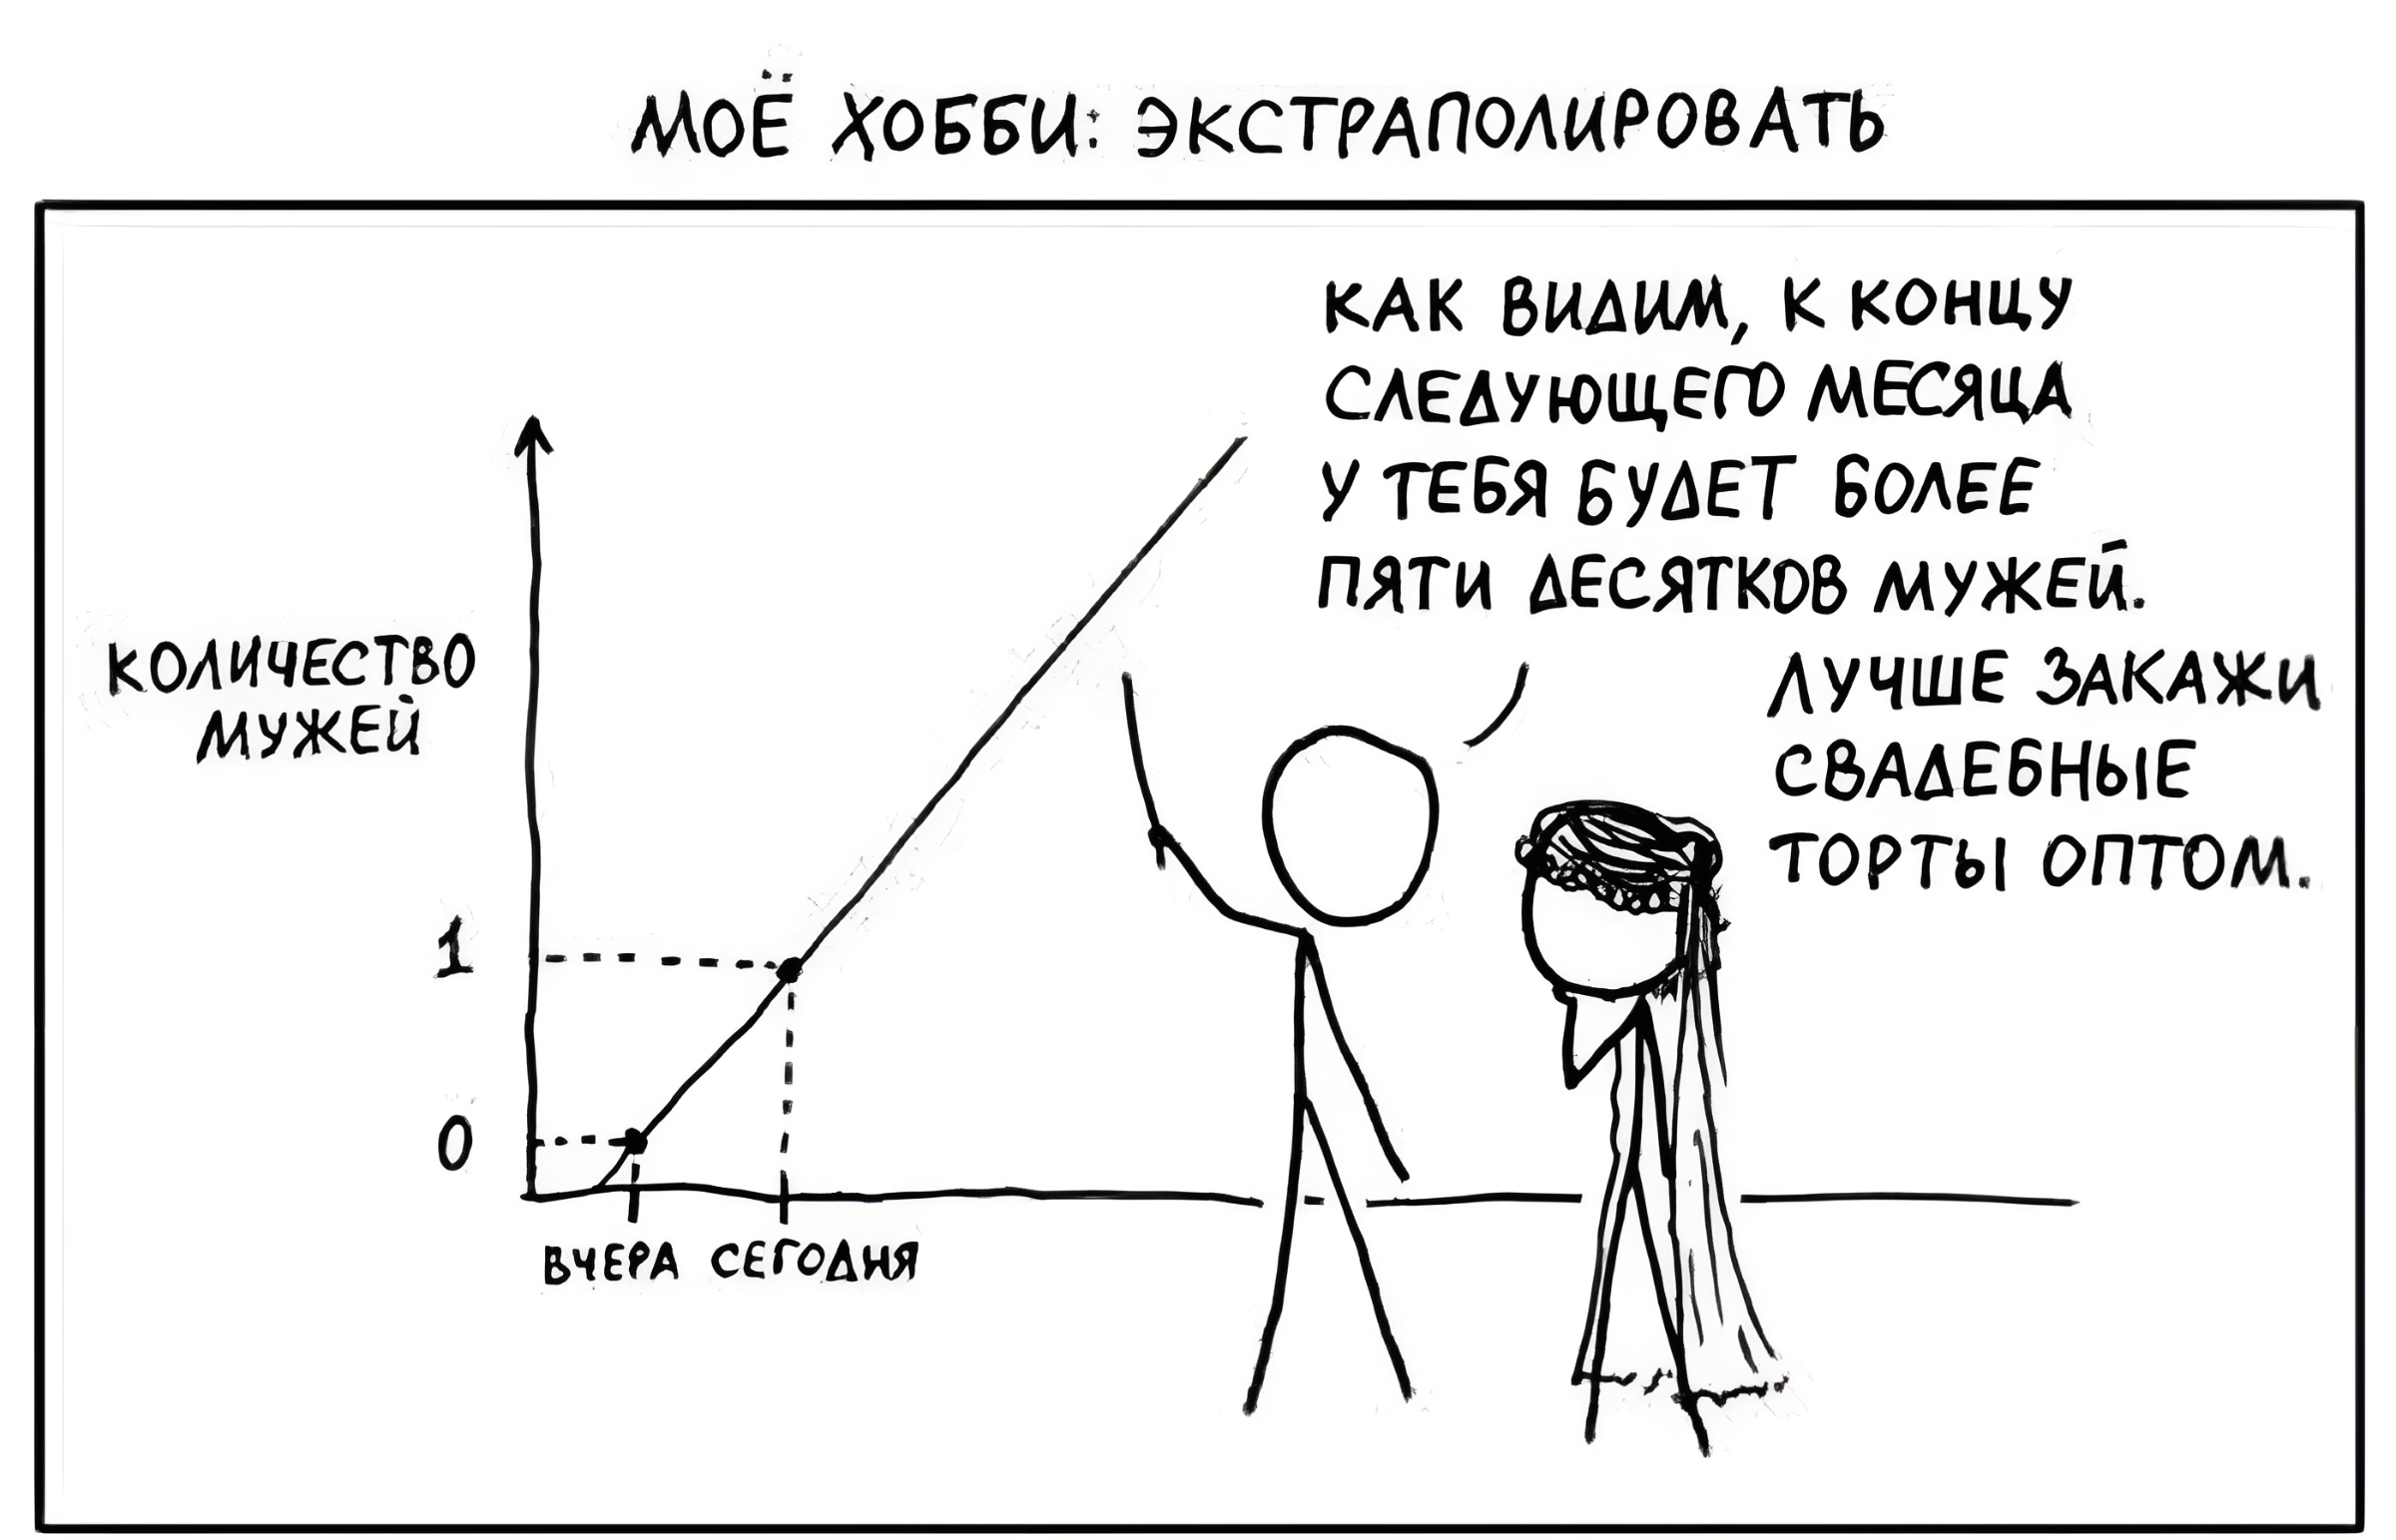
\includegraphics[width=0.875\linewidth]{meme.png}}
\end{figure}
\end{document}